\section{Appendix on Experimental Setup}\label{sec:apx-con:experimental_setup}

\subsection{Autoencoder Architecture}
For the encoder and decoder, we rely on a vanilla \glspl{CNN} implemented as a $\beta$-\gls{VAE}~\citep{kingma2014auto}.

\textbf{Encoder.} The encoder consists of two convolutional layers with kernel size $(3, 3)$ and stride $(1, 1)$ mapping to $16$, $32$, respectively.
The features are flattened and then passed to two linear layers with hidden dimension $256$ and $n_z$.
Each layer (except for the last) is followed by a layer norm~\citep{ba2016layer} and a LeakyReLU nonlinearity.

\textbf{Decoder.} The decoder first uses two linear layers to map to hidden dimensions of $256$ and $32768$, respectively.
We then apply two 2D transposed convolutions~\citep{dumoulin2016guide} reducing the number of channels first to $16$, and then to $1$.
Each layer (except for the last linear and last convolutional) is followed by a layer norm~\citep{ba2016layer} and a LeakyReLU nonlinearity.
Finally, we apply a sigmoid function to clip the output into the range $[-1, 1]$.

\subsection{Latent Dynamic Models}\label{sub:apx-con:latent_dynamic_models}
In the following section, we provide implementation details for the latent dynamic models that we evaluated as part of this work.

\subsubsection{Coupled Oscillator Network (CON)}\label{ssub:apx-con:latent_space_dynamic_models:con}
We leverage the \gls{CON} in $\mathcal{W}$-coordinates given by \eqref{eq:con:conw_dynamics} for learning latent space dynamics. 
Specifically, we consider the input-to-force mapping $g(u)) = B(u) \, u(t)$, where $B(u) \in \mathbb{R}^{n \times m}$ is parametrized by few-layer \gls{MLP}. We report results for two different sizes of the \gls{MLP}: one medium-sized variant consisting of five layers with a hidden dimension of $30$ and a small variant with two layers and a hidden dimension of $12$. In both cases, we use a hyperbolic tangent as a nonlinearity.


% \begin{figure}[hbt]
%     \centering
%     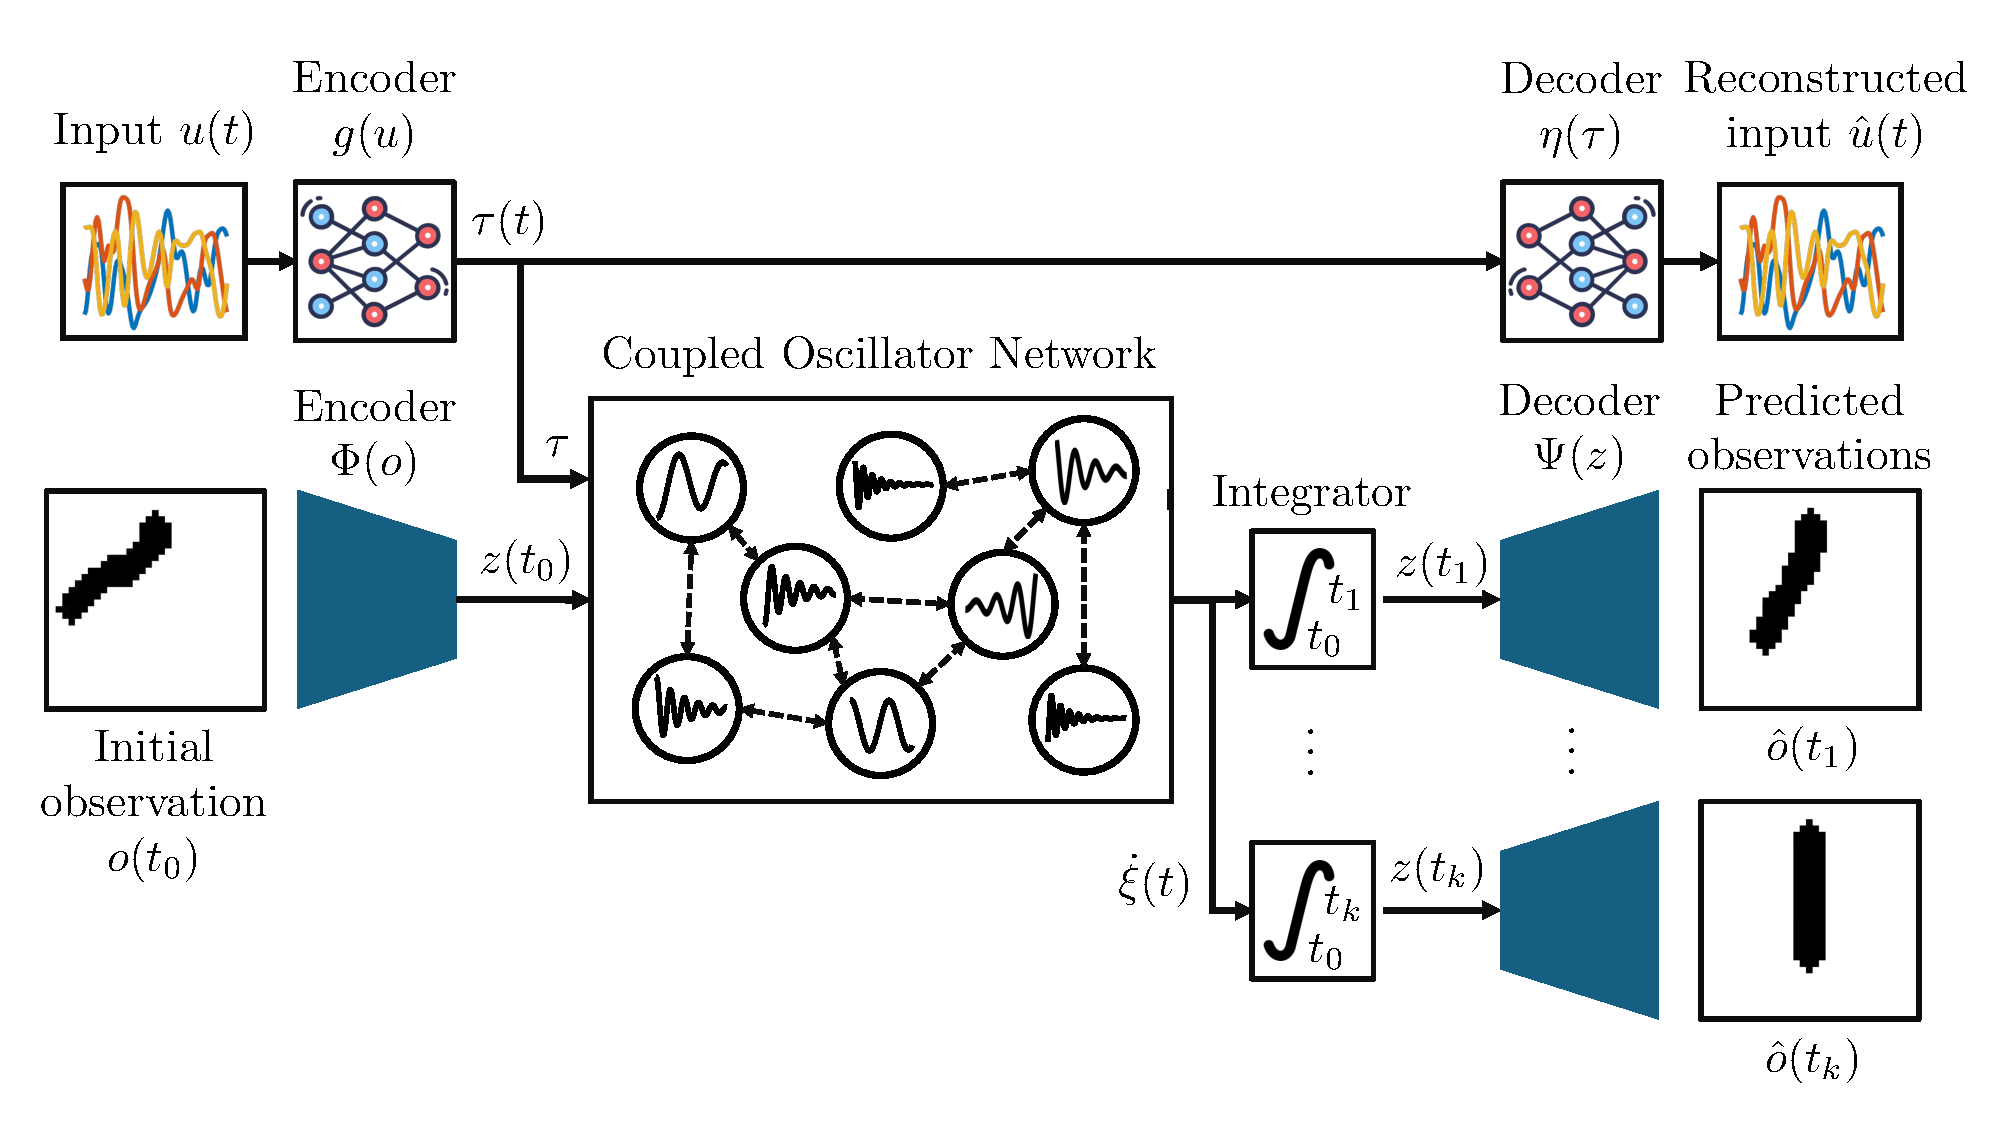
\includegraphics[width=1.0\columnwidth]{figures/autoencoder/blockdiagram_autoencoder_v1_cropped.pdf}
%     \caption{Exploiting \glspl{CON} for learning latent dynamics from pixels: We encode the initial observation $o(t_0)$ and the input $u(t)$ into latent space where we leverage the \gls{CON} to predict future latent states. Finally, we decode both the latent-space torques $\tau(t)$ and the predicted latent states $z(t)$.}
%     \label{fig:apx:blockdiagram_autoencoder}
% \end{figure}

When training the model, we jointly optimize $M_\mathrm{w}^{-1}, K_\mathrm{w}, D_\mathrm{w}, b$ and $g(u)$. 
However, we also need to make sure that we adhere to the stability constraints  $M_\mathrm{w}^{-1}, K_\mathrm{w}, D_\mathrm{w} \succ 0$. For this, we leverage the Cholvesky decomposition~\citep{petersen2008matrix}. Instead of directly learning the full matrix $A \in \mathbb{R}^{n_z \times n_z}$, we designate the elements of an upper triangular matrix $U \in \mathbb{R}^{n_z \times n_z}$ as the trainable parameters.
The Cholesky decomposition demands that $\mathrm{diag}(U_{11}, \dots, U_{n_z n_z}) > 0$. Therefore, we apply the operation
\begin{equation}
    U_{ii} = \log \left (1+ e^{\breve{U}_{ii} + \epsilon_1} \right ) + \epsilon_2,
\end{equation}
where $\breve{U}$ is the learned upper triangular matrix, and $\epsilon_1 = \num{1e-6}$ and $\epsilon_2 = \num{2e-6}$ are two small, positive values.
The positive-definite matrix $A$ is now given by $A = U^\top \, U \succ 0$.

\subsubsection{Neural ODEs}
We consider two kinds of Neural ODEs~\citep{chen2018neural}: the vanilla $f_\mathrm{NODE}: \xi(t) \times u(t) \mapsto \dot{\xi}(t)$ maps latent state and system actuation directly into a time derivative of the latent state. In contrast, for the \emph{MECH-NODE}, we enforce the latent dynamics to have a mechanical structure
\begin{equation}
    \dot{\xi}(t) = \begin{bmatrix}
        \frac{\mathrm{d} z}{\mathrm{d}t}\\
        \frac{\mathrm{d} \dot{z}}{\mathrm{d}t}
    \end{bmatrix} = \begin{bmatrix}
        \dot{z}(t)\\
        f_\mathrm{MECH-NODE}(\xi(t), u(t))
    \end{bmatrix}.
\end{equation}
We represent both $f_\mathrm{NODE}$ and $f_\mathrm{MECH-NODE}$ as \glspl{MLP} consisting of $5$ layers, a hidden dimension of $30$, and a hyperbolic tangent nonlinearity.

\subsubsection{Autoregressive models}

For the below stated autoregressive models, we divide the integration between two (latent) samples $\xi(t_k)$ and $\xi(t_{k+1})$ into $N_\mathrm{int}$ integration steps $\xi(t_k + \delta t), \dots, \xi(t_k + k' \delta t), \dots, \xi(t_k + N_\mathrm{int} \delta t)$ where $\delta t$ is the integration step size and $t_{k+1} = t_k + N_\mathrm{int} \delta t$. The autoregressive model now describes the transition $\xi(t_{k'+1}) = f_\mathrm{ar}(\xi(t_{k'}), u(t_k))) \: \forall k' \in 1, \dots, N_\mathrm{int}$.

\paragraph{RNN.}
We implement a standard, single-layer Elman RNN with \texttt{tanh} nonlinearity. The hidden state captures the latent state of the system. The latent state transition functions are given by
\begin{equation}
    \xi(t_{k'+1})
    % \begin{bmatrix}
    %     z(t_{k'+1})\\ \dot{z}(t_{k'+1})
    % \end{bmatrix}
    = \tanh(W_\mathrm{hh} \, \xi(t_{k'}) + b_\mathrm{hh} + W_\mathrm{ih} \, u(t_{k}) + b_\mathrm{ih}), 
\end{equation}
where $W_\mathrm{hh} \in \mathbb{R}^{2 n_z \times 2 n_z}$, $b_\mathrm{hh} \in \mathbb{R}^{2 n_z}$, $W_\mathrm{ih} \in \mathbb{R}^{2 n_z \times m}$, and $b_\mathrm{ih} \in \mathbb{R}^{2 n_z}$.

\paragraph{GRU.}
We implement a standard, single-layer GRU~\citep{cho2014learning} with \texttt{sigmoid} activation function where we interpret the latent state of the system as the hidden state of the cell. The latent state transition functions are given by
\begin{equation}
\begin{split}
    r =& \: \sigma \left ( W_\mathrm{hr} \, \xi(t_{k'}) + b_\mathrm{hr} + W_\mathrm{ir} \, u(t_{k}) + b_\mathrm{ir} \right )\\
    p =& \: \sigma \left ( W_\mathrm{hp} \, \xi(t_{k'}) + b_\mathrm{hp} + W_\mathrm{ip} \, u(t_{k}) + b_\mathrm{ip} \right )\\
    n =& \: \tanh \left ( r \odot \left ( W_\mathrm{hn} \, \xi(t_{k'}) + b_\mathrm{hn} \right) + W_\mathrm{in} \, u(t_{k}) + b_\mathrm{in} \right )\\
    \xi(t_{k'+1}) =& \: (1-p) \odot n + p \odot \xi(t_{k'})
\end{split}
\end{equation}
where $\sigma$ is the sigmoid function, $\odot$ the Hadamard product, $W_\mathrm{hr}, W_\mathrm{hp}, W_\mathrm{hn} \in \mathbb{R}^{2 n_z \times 2 n_z}$, $W_\mathrm{ir}, W_\mathrm{ip}, W_\mathrm{in} \in \mathbb{R}^{2 n_z \times m}$, and $b_\mathrm{hr}, b_\mathrm{ir}, b_\mathrm{ip}, b_\mathrm{in} \in \mathbb{R}^{2 n_z}$.

\paragraph{coRNN.} A time-discrete \gls{coRNN} is defined by the transition function
\begin{equation}
\begin{split}
    \xi(t_{k'+1}) = \begin{bmatrix}
        z(t_{k'+1})\\
        \dot{z}(t_{k'+1})
    \end{bmatrix} = \begin{bmatrix}
        z(t_{k'}) + \delta t \, \dot{z}(t_{k'})\\
        \dot{z}(t_{k'}) + \delta t \, \left ( - \gamma z(t_{k'}) - \varepsilon \dot{z}(t_{k'}) + \tanh \left ( W \xi(t_{k'}) + V u(t_k) + b \right ) \right )
    \end{bmatrix}
\end{split}
\end{equation}
where $\gamma, \varepsilon \in \mathbb{R}^+$ are positive, scalar hyperparameters representing the stiffness and damping coefficients, respectively. The term $\tanh \left ( W \xi(t_{k'}) + V u(t_k) + b \right )$ with $W \in \mathbb{R}^{2n_z \times 2n_z}$, $V \in \mathbb{R}^{n_z \times m}$, and $b \in \mathbb{R}^{n_z}$ contributes nonlinear state-to-state connections. It is implemented with a linear layer operating on $(\xi(t_{k'}), u(t_k))$ followed by a hyperbolic tangent nonlinearity.

\paragraph{CFA-CON.} We adapt the Alg.~\ref{alg:con:con_cfa} for predicting the time evolution in latent-space
\begin{equation}
    \xi(t_{k'+1}) = f_\mathrm{CFA-CON}(\xi(t_k'), u(t_k)),
\end{equation}
where $f_\mathrm{CFA-CON}$ describe the autoregressive state transition by the \gls{CFA-CON} model as introduced in Eq.~\ref{eq:con:cfa_con}.

\subsection{First-Order Variants of Dynamical Models}\label{sub:apx-con:1st_order_latent_dynamics}
For learning (latent) dynamics of \nth{1}-order systems (e.g., the reaction-diffusion dataset \emph{R-D}), it might be beneficial also to formulate the dynamical model to be of \nth{1}-order. 
While this is straightforward for some dynamics that do not explicitly take the order into account (e.g., RNN, GRU, NODE), for other models such as \gls{coRNN}, \gls{CON}, and \gls{CFA-CON} more adjustments are necessary.
Namely, we substitute the $\frac{\mathrm{d} z}{\mathrm{d}t}$ component of the \gls{ODE} with the expression for $\frac{\mathrm{d} \dot{z}}{\mathrm{d}t}$. Furthermore, we remove any terms that depend on the velocity $\dot{z}$ (e.g., damping effects).
Below, we report in detail the adapted, \nth{1}-order formulations for the \gls{coRNN}, \gls{CON}, and \gls{CFA-CON} models.

\paragraph{CON.} In the \nth{1}-order version, we adapt the standard, \nth{2}-order \gls{ODE} of the \gls{CON} network as defined in \eqref{eq:con:conw_dynamics} to
\begin{equation}
\begin{split}
    \dot{\xi}(t) = \dot{z}(t) = M_\mathrm{w}^{-1} \left ( g(u(t)) - K_\mathrm{w} z(t) - \tanh(z(t) + b) \right ).
\end{split}
\end{equation}

\paragraph{coRNN.} In the \nth{1}-order version, we define the transition function as
\begin{equation}
\begin{split}
    \xi(t_{k'+1}) = z(t_{k'+1}) = z(t_{k'}) - \delta t \, \gamma \, z(t_{k'}) + \delta t \, \tanh \left ( W \xi(t_{k'}) + V u(t_k) + b \right ).
\end{split}
\end{equation}

\paragraph{CFA-CON.}
We adapt a \nth{1}-order version of Alg.~\ref{alg:con:con_cfa} for predicting the time evolution in latent-space
\begin{equation}
\begin{split}
    \xi(t_{k'+1}) = z(t_{k'+1}) = z(t_{k'}) + \int_{t_{k'}}^{t_{k'} + \delta t} F(t_{k'}) - \kappa \, z(t')  \, \mathrm{d}t',\\
    F(t_{k'}) = g(u(t_{k})) - (K - \kappa) z(t_{k'}) - \tanh(W z(t_{k'}) + b),
\end{split}
\end{equation}
where the closed-form solution for the integral is given by
\begin{equation}
    \int_{t_{k'}}^{t_{k'} + \delta t} F(t_{k'}) - \kappa \, z(t')  \, \mathrm{d}t' = \frac{F(t_{k'})}{\kappa} \left ( 1 - \, e^{- \kappa \, \delta t} \right ).
\end{equation}

\subsection{Training}
We implement the network dynamics and the neural networks (e.g., encoder, decoder, and \glspl{MLP}) in JAX~\citep{jax2018github} and Flax~\citep{flax2020github}, respectively. When training or inferring time-continuous dynamical models (e.g., NeuralODE, CON), we rely on Diffrax~\citep{kidger2021neural} for numerical integration of the \gls{ODE} using the Dormand-Prince's 5/4 method~\citep{dormand1980family} (Dopri5). For the numerical integration of both the time-continuous and the time-discrete models (e.g., RNN, \gls{coRNN}, \gls{CFA-CON}), we use an integration time-step $\delta t$ of \SI{0.025}{s} and $\SI{0.01}{s}$ for the \emph{Toy Physics}~\citep{botev2021priors} and soft robotic datasets, respectively.

Because of the GPU memory constraints, we limit ourselves to a batch size of $30$ and $80$ trajectories for the \emph{Toy Physics}~\citep{botev2021priors} and soft robotic datasets, respectively.
We implement a learning rate schedule consisting of a warm-up (5 epochs) and a cosine annealing~\citep{loshchilov2016sgdr} period (remaining epochs). 
We employ an AdamW optimizer~\citep{kingma2014adam, loshchilov2018decoupled} with $\beta_1 = 0.9$, $\beta_2 = 0.999$ for updating both neural network weights (e.g., encoder, decoder) and parameters of the dynamical model (e.g., $K_\mathrm{}, D_\mathrm{w}$, $M_\mathrm{w}$, etc.).

\subsection{Evaluation Metrics}
Similar to other publications in the field~\citep{liu2018image, yu2018generative, stolzle2022reconstructing}, % more citations about evaluation metrics: \citep{yi2020cosmovae, yang2017high}
we state the \gls{RMSE}, the \gls{PSNR} and the \gls{SSIM}~\citep{wang2004image} between the ground-truth image $o \in \mathbb{R}^{h_\mathrm{o} \times w_\mathrm{o}}$ and the predicted image image $\hat{o} \in \mathbb{R}^{h_\mathrm{o} \times w_\mathrm{o}}$.
We use the separated test set for all evaluation results.

\subsubsection{Root Mean-Square Error}
The \gls{RMSE} between the two images is given by
\begin{equation}
    \text{RMSE}(o, \hat{o}) = \sqrt{\sum_{u = 1}^{h_\mathrm{o}} \sum_{v = 1}^{w_\mathrm{o}} \frac{(o_{uv} - \hat{o}_{uv})^2}{h_\mathrm{o} \, w_\mathrm{o}}}.
\end{equation}

\subsubsection{Peak Signal-to-Noise Ratio}
The \gls{PSNR} is a function of the total \gls{MSE} loss and the maximum dynamic range of the image $L$. 
\begin{equation}
    \mathrm{PSNR}(o, \hat{o}) = 20 \, \log_{10} (L) - 10 \, \log_{10} \left (\sum_{u = 1}^{h_\mathrm{o}} \sum_{v = 1}^{w_\mathrm{o}} \frac{(o_{uv} - \hat{o}_{uv})^2}{h_\mathrm{o} \, w_\mathrm{o}} \right ).
\end{equation}
As we work with normalized images with pixels in the interval $[-1, 1]$, the dynamic range is $L = 2$.
% It is important to mention that the \gls{PSNR} is not linearly accumulated over mini-batches but rather computed as a function of the \gls{MSE} loss over the entire dataset.

\subsubsection{Structural Similarity Index Measure}
As simple pixel-by-pixel metrics such as \gls{RMSE} or \gls{PSNR} tend to average out any encountered errors, this could lead to a situation in which a significant reconstruction error in a part of the image is not seen in the \gls{RMSE} metric but has a huge impact on the visual appearance of the reconstruction. \gls{SSIM}~\citep{wang2004image} incorporates not just the \emph{absolute errors}, but also the strong inter-dependencies between pixels, especially when they are spatially close.
The \gls{SSIM} metric between two observations $o$ and $\hat{o}$ is given by
\begin{equation}
    \mathrm{SSIM}(o, \hat{o}) = l^\alpha(o, \hat{o}) \, c^\beta(o, \hat{o}) \, s^\gamma(o, \hat{o}),
\end{equation}
where
\begin{equation}
    l(o, \hat{o}) = \frac{2 \mu_o \mu_{\hat{o}} + C_1}{\mu_o^2 + \mu_{\hat{o}}^2 + C_1},
    \quad
    c(o, \hat{o}) = \frac{2 \sigma_o \sigma_{\hat{o}} + C_2}{\sigma_o^2 + \sigma_{\hat{o}}^2 + C_2},
    \quad 
    s(o, \hat{o}) = \frac{\sigma_{o\hat{o}} + C_3}{\sigma_o \sigma_{\hat{o}} + C_3}.
\end{equation}
We use the constants $C_1 = (k_1 L)^2$, $C_2 = (k_2 L)^2$ and $C_3 = C_2 / 2$, where $L$ signifies the dynamic range as previously used for the \gls{PSNR} metric,
and $k_1 = 0.01$ and $k_2 = 0.03$. The average $\mu$ and the variance $\sigma^2$ is computed with a Gaussian filter with a 1D kernel of size $11$ and sigma $1.5$.
We set the weight exponents $\alpha$, $\beta$, and $\gamma$ for the luminance, contrast, and structure comparisons all to one.
We rely on the PIX library~\citep{deepmind2020jax} for efficiently computing the \gls{SSIM} metric.

\subsection{Compute Resources}\label{apx:sub:compute_resource}
% We train all models on a desktop workstation with a 12th-Gen i9 12900KF CPU with 16 cores, 64 GB of RAM, and an Nvidia GeForce RTX 3090 GPU with 24 GB of VRAM.

We trained the models on several desktop workstations for a total duration of roughly \SI{150}{h}.
In total, we relied on 10x RTX 3090/4090 GPUs, each with 24 GB of VRAM, training the models in parallel.
Each workstation contained between 64 and 128 GB of RAM, and we used roughly 100 GB of total storage. 
Training each model on one random seed took between \SI{45}{min} and \SI{4}{h} depending on the model type, the integration time constant, and the number of trainable parameters.
The hyperparameter tuning we conducted beforehand (only on one random seed) took roughly the same time and computational resources as generating the final results.

For the control experiments, we additionally used a laptop with a 16-core Intel Core i7-10870H CPU and 32 GB RAM. We did not need to use a GPU for evaluating the model during closed-loop control.